\section{Building pangenomic models}

\subsection{Constructing graphs} 
% Robin

\subsection{Indexing and succinct genome graph models}
% Jouni / Erik?

\subsection{Other population-ish succinct data structures}
% Erik / Jouni?

\subsubsection{de Bruijn}

\subsubsection{VCFs / genotype calls / haplotypes / binary matrices}

\subsubsection{Alignments / collections of strings}


\section{Finding structure in the model}

\subsection{Visualization}
% Adam

Once one has constructed a graph pangenomic model, one might want to look at it.
A number of tools have been developed for this purpose.

Bandage (\textbf{B}ioinformatics \textbf{A}pplication for \textbf{N}avigating \textit{\textbf{D}e novo} \textbf{A}ssembly \textbf{G}raphs \textbf{E}asily) \citep{Wick_2015} is one of the most popular \citep{Mikheenko_2019}.
Originally designed for working with bacterial assembly and meta-assembly graphs \citep{Wick_2015}, it supports a wide range of formats and graph  paradigms.
It can be effectively used for interactively visualizing and exploring subregions of human-scale pangenome graphs \citep{Garrison_2019}, but its shortcomings become apparent at larger scales or with higher degrees of connectivity between graph regions \citep{Mikheenko_2019}.
The tool does have support for restricting the portion of the graph displayed to a particular ``scope'', but the tool is fundamentally built around laying out the graph under study in two dimensions, with all nodes represented, and panning and zooming around it.
Moreover, while the tool includes the ability to search for sequences in the graph, it does not have any ability to structure graph display using known linearization information.
Additionally, Bandage is implemented as a cross-platform native C++/Qt application \citep{Wick_2015}, which allows the tool to be self-contained but precludes the use of cloud resources for dealing with larger graphs; all graph data must be stored and processed on the user's machine at visualization time.

GfaViz is another C++/Qt application for visualizing genome graphs which claims full support for newer GFA2 features, such as the gaps which allow GFA2 to represent scaffold graphs in addition to assembly graphs; these features are not available in Bandage, which supports only GFA1 \citep{Gonnella_2018}.
However, unlike Bandage, the GfaViz project has not released any binary builds or user interface screenshots of their application, so Bandage remains the more accessible tool.

Departing from the desktop application model, two recent graph visualization tools, \textbf{S}caffold \textbf{G}raph \textbf{T}ool\textbf{K}it (SGTK) and \textbf{A}ssembly \textbf{G}raph \textbf{B}rowser (AGB), adopt a build-a-web-page model, in which a web-based visualization is prepared that does not rely on further server support, lowering end-user system requirements \citep{Kunyavskaya_2018,Mikheenko_2019}.
SGTK is designed for visualizing scaffold graphs, which can have negative-overlap gaps between sequenced segments, and is based around the in-browser Cytoscape.js graph layout and rendering library \citep{Kunyavskaya_2018}.
It includes a potentially highly interpretable, reference-sequence-structured ``browser'' layout, but its use of Cytoscape.js appears to push it towards a generic circular node representation, rather than the noodles of Bandage \citep{Kunyavskaya_2018}.
Moreover, its authors do not demonstrate its usability on large graphs, with the largest graph evaluated having only 923 nodes and 60,679 edges \citep{Kunyavskaya_2018}.

AGB has a similar overall design to SGTK, but makes different implementation choices.
It is relatively tightly tied to the assembly graph use case, requiring each (sequence-bearing) edge to be classifiable as ``unique'' or ``repetitive'' based on assembler annotation or sequencing coverage \citep{Mikheenko_2019}.
Where SGTK used Cytoscape.js, AGB relies on the venerable \texttt{graphviz} tool itself, compiled for execution in the browser \citep{Mikheenko_2019, Ellson_2001}.
This lets it lay out graphs in a more flow-guided way, using graphviz's rank-based algorithms, as compared to Cytoscape.js's more force-directed-looking layouts \citep{Mikheenko_2019, Kunyavskaya_2018}.
AGB is built around the idea of splitting up an assembly graph and visualizing portions of it, and features many ways to do this, including linear-reference-based and minimum-edge-cut-based approaches \citep{Mikheenko_2019}.
On the backend, the tool is built around potentially megabyte-scale JSON files \footnote{\url{https://github.com/almiheenko/almiheenko.github.io/blob/8f4b2f8c7c498f04fa32f53f69b4bc59888a14f0/AGB/Flye_Human/data/repeat_graph.json}}, with no apparent provision for region-specific download, but the tool is still demonstrated to be scalable enough to handle human and other eukaryotic assembly graphs \citep{Mikheenko_2019}.

There is a difference in scale when moving from an assembly or scaffold graph to a comprehensive pangenome graph for even a species with as little diversity as humans.
While tools like SGTK and AGB have been demonstrated on graphs with tens of thousands of entities, the 1000 Genomes Project dataset contains 88 million known human variants \citep{1000_2015}, which gives a density over the 3 billion base human genome of about 34 bases per variant, and a comprehensive pangenome graph with tens to hundreds of millions of elements---a much larger graph than those that SGTK and AGB have been shown to work with.
Moreover, to achieve their single-megabyte-scale visualization file sizes for hundred-megabase- to gigabase-scale assemblies, these tools necessarily elide sequence information.

To deal with comprehensive pangenome graphs with sequence data, one design approach is to keep the browser-based client but to put more intelligence into the server.
This is the avenue taken by the Sequence Tube Map, which renders regions of pangenome graphs using a visual language inspired by transit system maps \citep{Beyer_2019}.
This tool operates at a much more magnified zoom level than tools designed to work with assembly graphs, and is useful for visualizing base-scale variation and short read mapping locations in human-chromosome-scale graphs \citep{Beyer_2019}.
However, its imposition of a local linear ordering and its limited graph simplification tools make it difficult to use on larger regions \citep{Beyer_2019}.
Additionally, its architectural decision to load the graph from disk for every request makes latency prohibitively high when working with combiend graphs above the scale of a single chromosome, so the tool is not suitable for graphs which cannot be broken up into chromosome-scale connected components.

Other approaches to visualizing comprehensive pangenome graphs rely on restricting the problem in order to improve efficiency.
For example, by forcing the sequence-bearing nodes of the graph into a one-dimensional layout, and producing vector rather than raster output, the \texttt{vg viz} tool promises to render graphs of arbitrary size and complexity in linear time \citep{Garrison_2019}. The intended use case seems to be to use a single global linearization, and to interactively render regions of it for display, but it is also possible to non-interactively render an entire graph to a very large image \citep{Garrison_2019}. The tool is designed around a base-level visual representation of the graph, and optimized for comparing long embedded paths in the graph, on the basis of which nodes they do or do not visit \citep{Garrison_2019}. However, as with the Sequence Tube Map, it can be difficult to understand high-level or nonlinear structures in such a linearized layout \citep{Garrison_2019}. In contrast to the Sequence Tube Map no provision is made for visualizing short read alignments \citep{Garrison_2019}.

Figure~\ref{fig:visualization} provides a visual overview of the visualization methods surveyed here. It remains an open problem to interactively visualize a comprehensive human pangenome graph, potentially including interchromosomal connections, at a variety of zoom levels, with modestly provisioned end-user hardware.

\begin{figure}[h]
    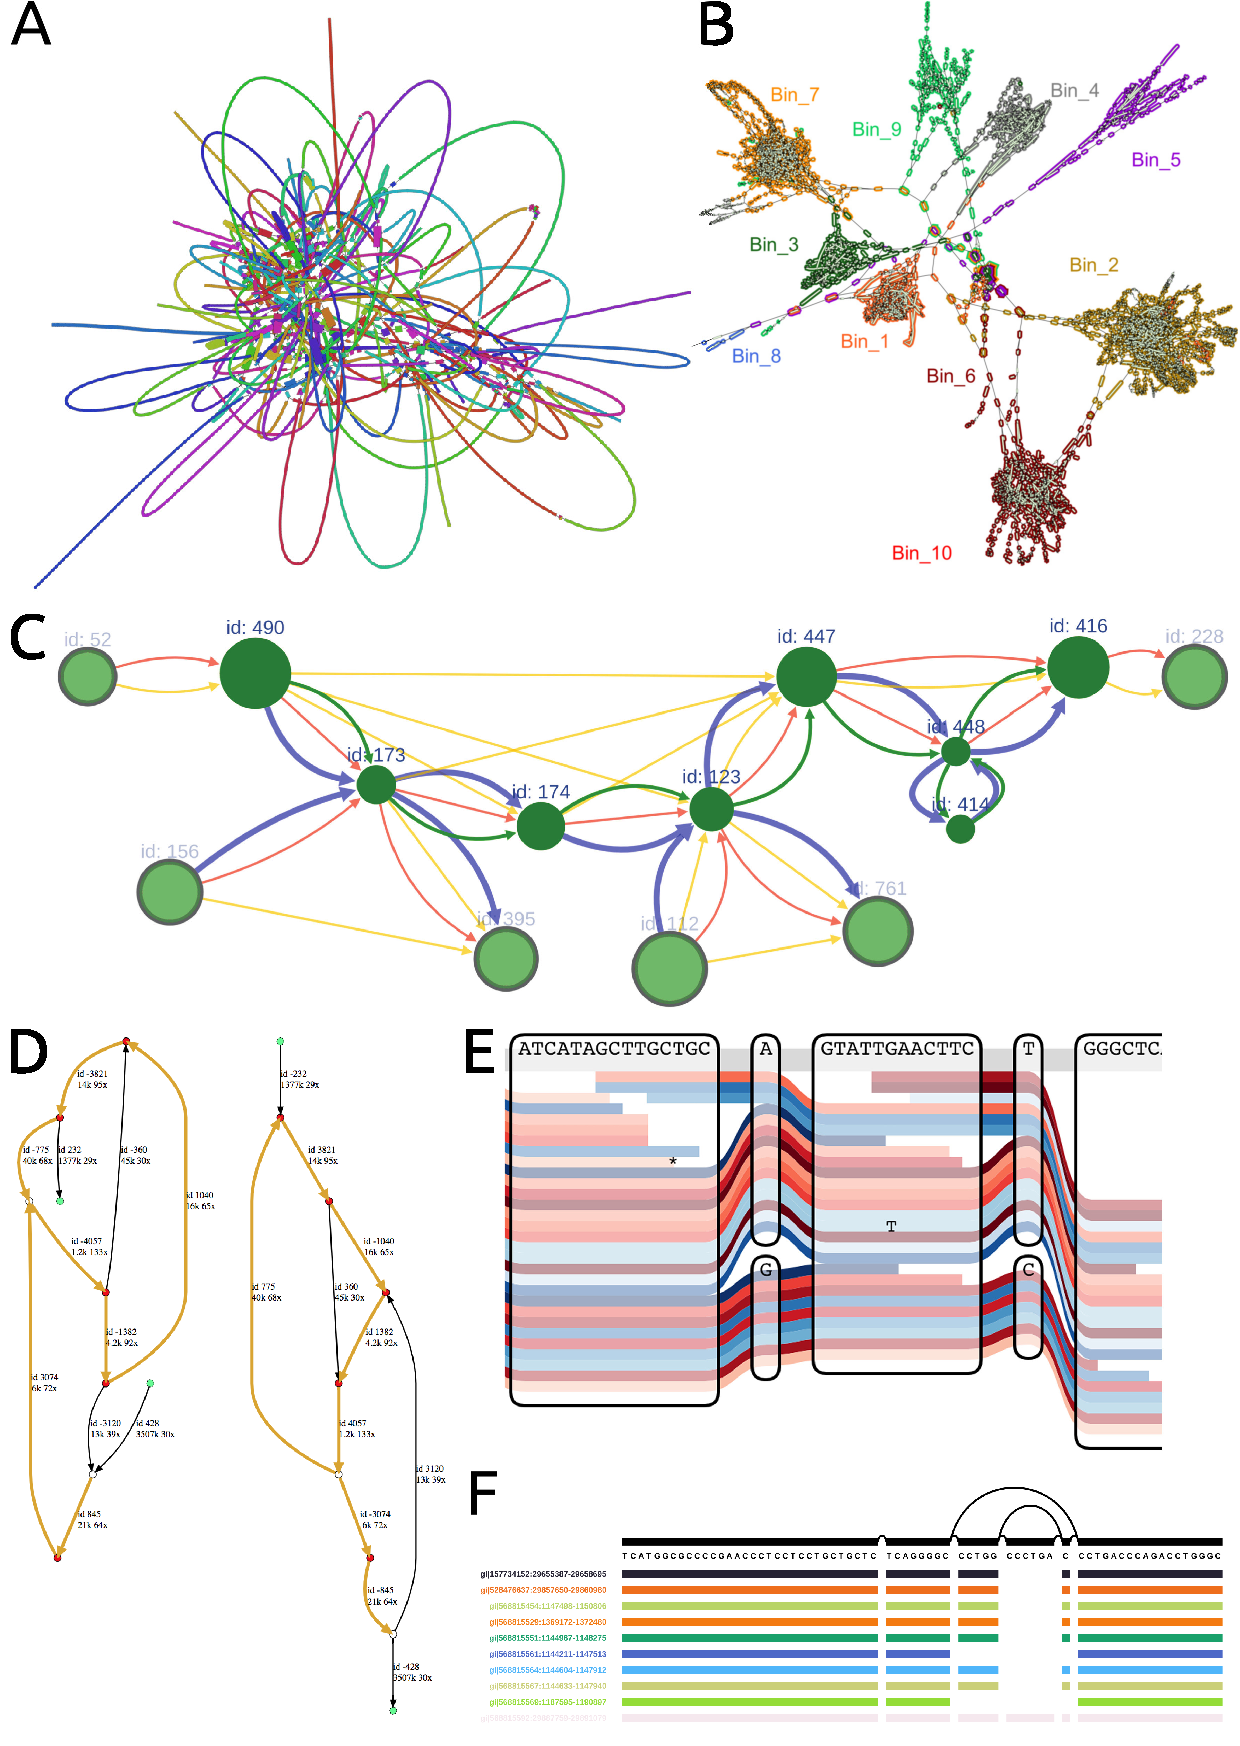
\includegraphics[width=0.9\textwidth]{figures/visualization.eps}
    \caption{\label{fig:visualization} An overview of several approaches to visualizing assembly, scaffold, and comprehensive pangenome graphs. \textbf{A:} Bandage, adapted from \cite{Wick_2015} supplementary section~6. \textbf{B:} GfaViz, adapted from \cite{Gonnella_2018} supplementary figure~S4. \textbf{C:} SGTK, adapted from \cite{Kunyavskaya_2018} figure~1. \textbf{D:} AGB, adapted from \cite{Mikheenko_2019} figure~S3. \textbf{E:} Sequence Tube Map, adapted from \cite{Beyer_2019} figure~2. \textbf{F:} \texttt{vg viz}, adapted from \cite{Garrison_2019} figure~2.20.}
\end{figure}

% Go back and talk about ABySS-Explorer (2009) and its "polar" graphs and wiggly sequence edges?
% Bandage: cross-platform native application
    % Versatile and popular
    % Client-only
    % Could look up a reference but not view vs it
% GfaViz: C++/Qt tool with full GFA1/2 support
    % Has a GUI but no screenshots or binaries
    % Can show cool stuff like reads connected to their assembly contigs
% SGTK
    % build-view model
    % Cytoscape.js or genome browser linear-structured
    % designed for scaffold graphs (more processed?)
    % Not proven on large graphs; only shown going up to 100s of nodes
% AGB: auto-subgraphs (to 100 nodes) and simplifies assembly graphs
    % js GraphViz based
    % Still uses a build-web-page model
    % Kind of tied to assemblies (notion of repetitive vs non-repetitive edges)
    % Can view vs a reference
    % Scales to C elegans at least
        % O(300 * 100 = 30000) nodes
    % Appears to be structured around megabyte-scale GraphViz graphs https://github.com/almiheenko/almiheenko.github.io/tree/master/AGB
        % No LOD-ing on the backend for efficient download, but not a problem at the scale of 10s of thousands.
% Tube Map
    % Client-server model: requires a server, but can use server resources to crunch the graph
    % Designed to impose a left to right local ordering that orients the edges in a hopefully sensible way
    % Scales well to millions of nodes, demonstrated on partial human pangenome graph references


%\citep{Wick_2015} : Bandage
%\citep{Gonnella_2018} : GfaViz
%\citep{Kunyavskaya_2018} : SGTK
%\citep{Mikheenko_2019} : AGB
%\citep{Beyer_2019} : TubeMap
%\citep{Garrison_2019} : Thesis

\subsection{Finding structures in pan-genome graphs}
% Jordan

